\documentclass[11pt,a4paper]{article}
\usepackage[utf8]{inputenc}
\usepackage[T1]{fontenc}
\usepackage{amsmath,amsfonts,amssymb}
\usepackage{graphicx}
\usepackage{xcolor}
\usepackage{booktabs}
\usepackage{array}
\usepackage{hyperref}
\usepackage{tikz}
\usetikzlibrary{arrows.meta,positioning,fit,backgrounds,calc}
\usepackage{fancybox}
\usepackage{enumitem}

\definecolor{darkblue}{RGB}{0,51,102}
\definecolor{priceblue}{RGB}{0,102,204}
\newcommand{\blue}[1]{\textcolor{priceblue}{\textbf{#1}}}
\newcommand{\gc}{\textbullet}

\begin{document}

\section*{\centering Industrial FM-to-C-band Spectrum-Sensing Node}
\noindent
\section*{SDR and Processing Backend Selection}

The revised platform is a modular single-channel spectrum-sensing node for
approximately 70~MHz to 6~GHz monitoring. Compared with the earlier
USRP~N210-based dual-branch concept, this version adopts an
\textbf{industrial-ready, single-RX architecture} centered on a
\textbf{USRP B200mini-i} and a \textbf{Jetson Orin Nano 8GB}. The change keeps
full FM-to-C-band frequency coverage while reducing daughterboard cost,
simplifying synchronization, and aligning the design with currently available
hardware.

\medskip
\noindent
\textit{USRP B200mini-i Industrial SDR.}
\begin{itemize}
	\item The B200mini-i provides integrated RF coverage from
	\textbf{70~MHz to 6~GHz} through the AD9361 transceiver, avoiding the external
	daughterboard stack required by the legacy N210 solution. In this design it is
	used as a \textbf{single receive sensing front-end} with approximately
	\textbf{56~MHz instantaneous bandwidth}, \textbf{12-bit conversion}, and
	USB~3.0 host connectivity.
	\item \textbf{Industrial deployment advantage:} the B200mini-i can be integrated
	into a ruggedized enclosure and is specified for \textbf{-40~$^\circ$C to
	+75~$^\circ$C} operation in the industrial configuration, which is a major
	advantage over used, non-industrial legacy SDRs.
	\item \textbf{Key trade-off versus the old N210 architecture:} this design gives
	up simultaneous dual-branch reception. Instead, the node time-shares a
	single RF path through antenna and filter switching. This reduces RF hardware
	cost and still supports wideband scanning missions.
	\item Estimated price: \blue{1,100--1,400 USD} for the SDR plus industrial
	enclosure kit.
	\item \textbf{Open-source software support:} UHD remains the primary driver
	stack, with compatibility for GNU Radio, Python, C/C++, and SoapySDR-based
	workflows.
\end{itemize}

\noindent
\textit{Jetson Orin Nano 8GB.}
\begin{itemize}
	\item The processing backend is upgraded from Jetson Nano 4GB to
	\textbf{Jetson Orin Nano 8GB}, reflecting current availability and a much
	stronger compute margin for field analytics, signal classification, and future
	edge-AI workflows.
	\item Key specifications: \textbf{6-core ARM Cortex-A78AE}, \textbf{8~GB LPDDR5},
	Gigabit Ethernet, multiple USB~3.0 ports, and 40-pin GPIO for switch and
	attenuator control.
	\item Power envelope: approximately \textbf{15--25~W} depending on operating
	mode and workload. This is higher than the legacy Jetson Nano 4GB, but it
	enables substantially more on-node processing headroom.
	\item \textbf{System-level consequence:} because the B200mini-i is USB-only, the
	Orin Nano must be \textbf{co-located in the same enclosure} as the SDR. The
	Jetson then serves as the edge gateway, forwarding processed spectra and
	metadata over Ethernet to the network.
	\item Estimated price: \blue{499--599 USD}.
\end{itemize}

\subsection*{Antenna System Configuration and RF Path Planning}

Because the revised architecture uses a single sensing RX chain, the antenna and
front-end planning changes from two simultaneous branches to one switched path:
\begin{center}
\small
\textit{Selected antenna}
\(\rightarrow\)
\textit{protection}
\(\rightarrow\)
\textit{preselector bank}
\(\rightarrow\)
\textit{LNA/bypass}
\(\rightarrow\)
\textit{programmable attenuation}
\(\rightarrow\)
\textit{USRP B200mini-i RX}
\end{center}

The earlier document separated VHF/UHF and UHF--C-band into parallel hardware
branches. In the updated design, those bands remain covered, but they share one
RF chain through solid-state switching. This is the main architectural shift
introduced by the research context.

\begin{center}
	\fcolorbox{red!33}{gray!15}{%
		\parbox{0.86\textwidth}{\centering\small
			BicoLOG 5070 or equivalent VHF/UHF antenna
			\(\rightarrow\)
			MSW-2-50DR+ antenna switch
			\(\rightarrow\)
			Limiter / ESD / DC block\\
			\(\rightarrow\)
			shared filter bank
			\(\rightarrow\)
			LNA / bypass
			\(\rightarrow\)
			ZX76-31R75PP-S+ attenuator
			\(\rightarrow\)
			B200mini-i RX
		}
	}
\end{center}

\begin{center}
	\fcolorbox{red!33}{gray!15}{%
		\parbox{0.86\textwidth}{\centering\small
			HyperLOG 7060 or equivalent UHF--C-band antenna
			\(\rightarrow\)
			MSW-2-50DR+ antenna switch
			\(\rightarrow\)
			Limiter / ESD / DC block\\
			\(\rightarrow\)
			shared filter bank
			\(\rightarrow\)
			LNA / bypass
			\(\rightarrow\)
			ZX76-31R75PP-S+ attenuator
			\(\rightarrow\)
			B200mini-i RX
		}
	}
\end{center}

\begin{table}[htbp]
	\centering
	\small
	\resizebox{\textwidth}{!}{%
	\begin{tabular}{@{}p{2.7cm}p{2.4cm}p{3.2cm}p{2.6cm}p{3.6cm}@{}}
		\toprule
		\textbf{Band} &
		\textbf{Antenna Type} &
		\textbf{Model Example} &
		\textbf{Frequency Range} &
		\textbf{Notes} \\
		\midrule

		VHF/UHF survey &
		Biconical &
		Aaronia BicoLOG 5070 &
		70~MHz--700~MHz &
		Preferred calibrated low-band antenna. \\

		UHF--C-band survey &
		Log-periodic &
		Aaronia HyperLOG 7060 &
		700~MHz--6~GHz &
		Main upper-band survey antenna. \\

		Low-cost alternative &
		Discone + log-periodic &
		Generic discone + HyperLOG &
		100~MHz--3~GHz plus 700~MHz--6~GHz &
		Lower cost, but reduced low-band confidence below 100~MHz. \\

		\bottomrule
	\end{tabular}
	}
	\caption{Antenna selection for the updated single-channel industrial node.}
	\label{tab:antenna-selection}
\end{table}

\subsection*{Supporting Hardware}

\begin{center}
\small
\textit{Prototype focus:} single shared RF chain, switched antennas, shared
filter bank, essential automation.
\end{center}
\begin{center}
\small
\textit{Field-ready focus:} industrial enclosure, programmable attenuation,
remote telemetry, thermal and power hardening.
\end{center}

\begin{enumerate}[label=\roman*)]

	\item \textbf{Antenna switching and protection.}

	The B200mini-i architecture benefits from a simple front-end antenna selection
	stage because only one receive path is active at a time. A practical baseline is
	a \textbf{Mini-Circuits MSW-2-50DR+} or equivalent \textbf{SPDT} RF switch
	between the low-band and high-band survey antennas. The switch is attractive
	because its \textbf{3.3V CMOS control} is compatible with Jetson GPIO, which
	keeps the control scheme close to the simpler GPIO-driven philosophy already
	present in the older design files.

	Protection should remain the first RF element after the selected antenna. The
	research context recommends a limiter/ESD stage built around a gas-discharge
	arrestor, TVS protection, and DC blocking so the shared front-end is not exposed
	directly to outdoor transients.

	\item \textbf{Preselection and band plan.}

	Although the B200mini-i tunes from 70~MHz to 6~GHz, the integrated transceiver
	does not remove the need for external selectivity. In the revised single-channel
	architecture, the filter bank becomes a \textbf{shared switched preselector}
	rather than one network per branch. This preserves the same monitoring regions
	discussed in the earlier draft, but with lower hardware duplication.

	\begin{table}[htbp]
		\centering
		\small
		\resizebox{\textwidth}{!}{%
		\begin{tabular}{p{2.5cm}p{3.6cm}p{2.4cm}p{1.6cm}p{4.7cm}}
			\toprule
			\textbf{Sensing Region} &
			\textbf{Suggested Filter Path} &
			\textbf{Nominal Band} &
			\textbf{Typ. IL} &
			\textbf{Purpose and Comments} \\
			\midrule

			70--88~MHz &
			Low-VHF path or broad VHF preselector &
			70--88~MHz &
			TBD &
			Supports lower-VHF sensing beneath the FM broadcast band. \\

			88--108~MHz &
			Switchable FM notch or FM pass &
			88--108~MHz &
			$<$1.5~dB pass &
			Protects the receiver during surveys, but can be bypassed when FM is the
			target band. \\

			108--700~MHz &
			Mini-Circuits SHP-50+ + SLP-750+ &
			108--700~MHz &
			$\sim$2~dB &
			General VHF/UHF preselection before amplification. \\

			700--960~MHz &
			Modular BPF or cavity filter &
			700--960~MHz &
			$<$2~dB &
			Useful for upper-UHF, public-safety, and telemetry regions. \\

			1.7--2.7~GHz &
			Custom BPF or VBFZ-2130-S+ style path &
			1.7--2.7~GHz &
			$<$2~dB &
			Targets cellular, ISM, and related microwave services. \\

			\textbf{3.0--4.2~GHz} &
			\textbf{Mini-Circuits SBP-3800+} &
			\textbf{3.0--4.2~GHz} &
			\textbf{$<$3~dB} &
			\textbf{Concrete catalog part retained from the research note to close the
				3--4~GHz gap.} \\

			4.0--6.0~GHz &
			Marki Microwave C-band BPF or equivalent &
			4.0--6.0~GHz &
			$<$3~dB &
			Replaceable upper-band module for focused C-band sensing. \\

			\bottomrule
		\end{tabular}
		}
		\caption{Shared RF band plan for the B200mini-i single-channel sensing node.}
		\label{tab:rf-band-plan}
	\end{table}

	A deployable implementation can realize this bank using a compact \textbf{SP6T}
	or a cascaded solid-state switch arrangement built from parts in the same class
	as the \textbf{MSW-2-50DR+}. The earlier prototype idea of manual patch-cord
	routing remains acceptable for bench validation, but the research-backed field
	version assumes automated selection.

	\item \textbf{LNA and bypass strategy.}

	The gain plan remains frequency dependent, but it is now centralized into one
	shared chain. This reduces the number of active RF modules relative to the old
	dual-branch draft.

	\begin{table}[!ht]
		\centering
		\small
		\resizebox{\textwidth}{!}{%
		\begin{tabular}{p{4.2cm}p{2.3cm}p{1.7cm}p{1.5cm}p{4.6cm}}
			\toprule
			\textbf{Model} &
			\textbf{Range} &
			\textbf{Gain} &
			\textbf{NF} &
			\textbf{Use Case} \\
			\midrule

			Mini-Circuits ZX60-33LN-S+ &
			50~MHz--3~GHz &
			20~dB &
			3~dB &
			Main LNA path for VHF, UHF, and lower microwave sensing. \\

			Optional 3--4~GHz LNA &
			3.0--4.2~GHz &
			15--25~dB &
			TBD &
			Optional gain flattening path when the 3--4~GHz region is mission-critical. \\

			Amplitech AGLNA035082 &
			4.0~GHz--8.0~GHz &
			26~dB typ. &
			0.9~dB &
			C-band and upper microwave amplification path. \\

			Bypass path &
			DC--6~GHz class &
			0~dB &
			-- &
			Allows protected operation near strong emitters and prevents unnecessary
			compression. \\

			\bottomrule
		\end{tabular}
		}
		\caption{Frequency-dependent gain options for the shared RF chain.}
		\label{tab:lna-selection}
	\end{table}

	The LNA stage should be placed after the selected preselector path, not before
	it, so strong out-of-band signals are attenuated prior to gain. In a compact
	deployable version, the Jetson GPIO can command the LNA/bypass state in the same
	way that the older design used GPIO for RF switching.

	\item \textbf{Attenuation strategy.}

	The research context strongly favors a programmable attenuator for field use,
	because a single unattended node must adapt to both quiet rural environments and
	high-power urban RF scenes. The selected part is:

	\begin{itemize}
		\item \textbf{Mini-Circuits ZX76-31R75PP-S+}: \textbf{0--31.5~dB} in
		\textbf{0.5~dB steps}, DC--6~GHz class. Estimated:
		\blue{300--350 USD}.
	\end{itemize}

	This is a meaningful departure from the earlier prototype approach that relied on
	manual fixed SMA pads. The fixed-pad idea is still valid for laboratory
	prototyping, but the new document assumes a more deployable baseline where
	remote gain control is part of the default hardware stack.

	\item \textbf{Timing and synchronization.}

	The B200mini-i can operate from its onboard reference for many scanning tasks,
	but the updated architecture still benefits from an external timing option when
	metadata consistency or multi-node comparison matters.

	\begin{itemize}
		\item \textbf{External reference input:} 10~MHz and 1~PPS via SMA.
		\item \textbf{Suggested source:} Leo Bodnar GPSDO or equivalent compact GPSDO
		module. Estimated: \blue{50--150 USD}.
		\item The node software should log reference-lock and GPS-lock state alongside
		capture metadata.
	\end{itemize}

\end{enumerate}

\subsection*{System Block Diagram}

The following diagram summarizes the revised single-channel industrial node. It
keeps the component-selection flavor of the original document, but reflects the
research-backed B200mini-i + Orin Nano architecture.

\begin{center}
	\resizebox{\textwidth}{!}{%
	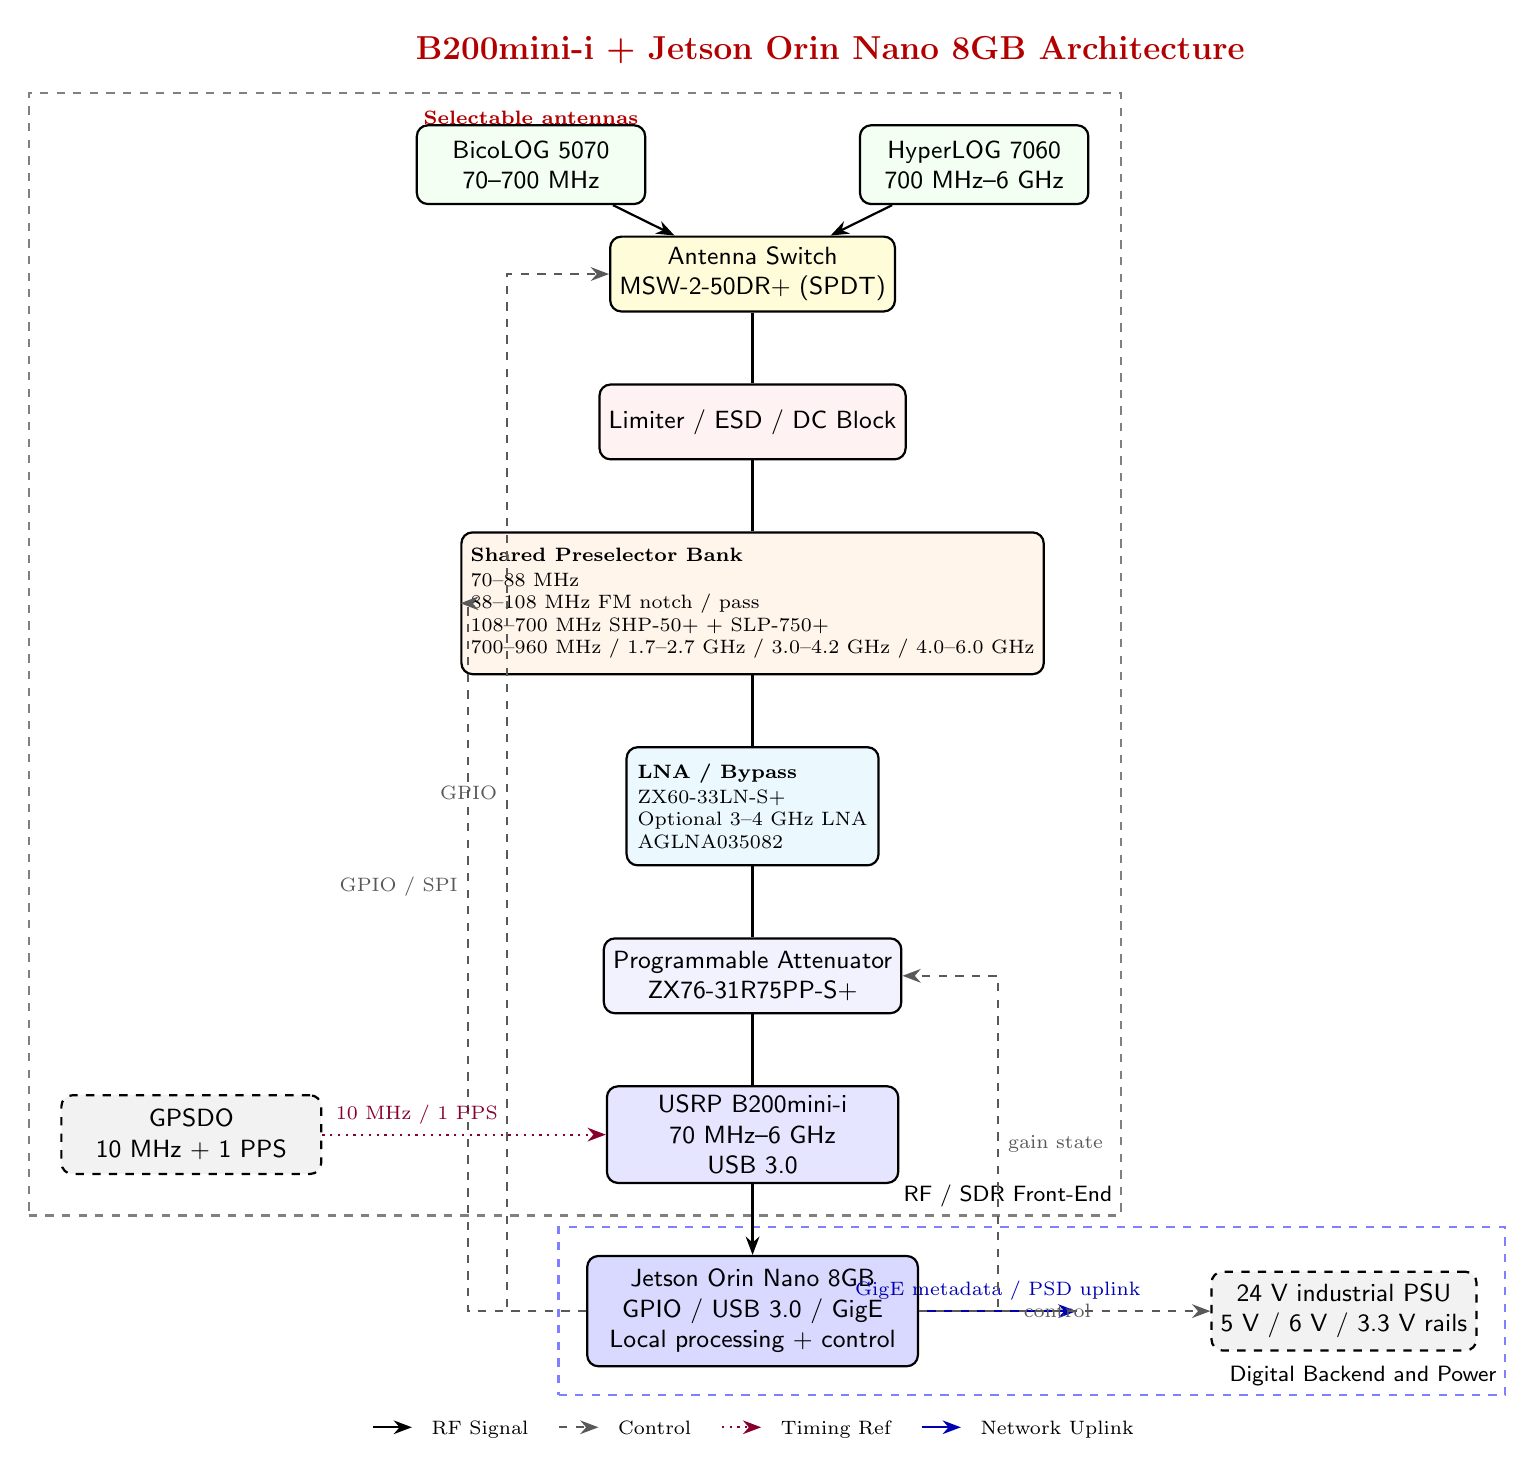
\begin{tikzpicture}[
		font=\small\sffamily,
		>=Stealth,
		antblock/.style={draw, thick, fill=green!5, rounded corners, minimum height=1.0cm, minimum width=2.9cm, align=center},
		protblock/.style={draw, thick, fill=red!5, rounded corners, minimum height=0.95cm, minimum width=3.2cm, align=center},
		switchblock/.style={draw, thick, fill=yellow!15, rounded corners, minimum height=0.95cm, minimum width=3.2cm, align=center},
		filterblock/.style={draw, thick, fill=orange!8, rounded corners, minimum height=1.8cm, minimum width=4.0cm, align=left, font=\scriptsize},
		lnablock/.style={draw, thick, fill=cyan!8, rounded corners, minimum height=1.5cm, minimum width=3.2cm, align=left, font=\scriptsize},
		attblock/.style={draw, thick, fill=blue!5, rounded corners, minimum height=0.95cm, minimum width=3.2cm, align=center},
		sdrblock/.style={draw, thick, fill=blue!10, rounded corners, minimum height=1.2cm, minimum width=3.7cm, align=center},
		procblock/.style={draw, thick, fill=blue!15, rounded corners, minimum height=1.4cm, minimum width=4.2cm, align=center},
		powerblock/.style={draw, thick, fill=gray!10, dashed, rounded corners, minimum height=1.0cm, minimum width=3.3cm, align=center},
		annot/.style={font=\scriptsize\bfseries, text=red!70!black},
		arrow/.style={thick,->},
		ctrlarrow/.style={thick,dashed,->,gray!70!black},
		refarrow/.style={thick,dotted,->,purple!70!black},
		etharrow/.style={thick,->,blue!70!black},
		node distance=0.9cm and 1.2cm
		]

		\node[font=\large\bfseries,text=red!70!black] at (6.0,10.4)
		{B200mini-i + Jetson Orin Nano 8GB Architecture};

		\node[annot] at (2.2,9.55) {Selectable antennas};
		\node[antblock] (ant1) at (2.2,8.95) {BicoLOG 5070\\70--700 MHz};
		\node[antblock,right=2.7cm of ant1] (ant2) {HyperLOG 7060\\700 MHz--6 GHz};
		\node[switchblock,below=of $(ant1)!0.5!(ant2)$] (antsw) {Antenna Switch\\MSW-2-50DR+ (SPDT)};
		\node[protblock,below=of antsw] (protect) {Limiter / ESD / DC Block};
		\node[filterblock,below=of protect] (filters) {
			\textbf{Shared Preselector Bank}\\[1pt]
			70--88 MHz\\
			88--108 MHz FM notch / pass\\
			108--700 MHz SHP-50+ + SLP-750+\\
			700--960 MHz / 1.7--2.7 GHz / 3.0--4.2 GHz / 4.0--6.0 GHz
		};
		\node[lnablock,below=of filters] (lna) {
			\textbf{LNA / Bypass}\\[1pt]
			ZX60-33LN-S+\\
			Optional 3--4 GHz LNA\\
			AGLNA035082
		};
		\node[attblock,below=of lna] (att) {Programmable Attenuator\\ZX76-31R75PP-S+};
		\node[sdrblock,below=of att] (sdr) {USRP B200mini-i\\70 MHz--6 GHz\\USB 3.0};
		\node[procblock,below=of sdr] (jetson) {Jetson Orin Nano 8GB\\GPIO / USB 3.0 / GigE\\Local processing + control};
		\node[powerblock,left=3.6cm of sdr] (gpsdo) {GPSDO\\10 MHz + 1 PPS};
		\node[powerblock,right=3.7cm of jetson] (psu) {24 V industrial PSU\\5 V / 6 V / 3.3 V rails};

		\draw[arrow] (ant1) -- (antsw);
		\draw[arrow] (ant2) -- (antsw);
		\draw[arrow] (antsw) -- (protect) -- (filters) -- (lna) -- (att) -- (sdr) -- (jetson);
		\draw[etharrow] (jetson.east) -- ++(2.0,0) node[midway,above,font=\scriptsize] {GigE metadata / PSD uplink};
		\draw[ctrlarrow] (jetson.west) -- ++(-1.0,0) |- node[pos=0.25,left,font=\scriptsize] {GPIO} (antsw.west);
		\draw[ctrlarrow] (jetson.west) -- ++(-1.5,0) |- node[pos=0.3,left,font=\scriptsize] {GPIO / SPI} (filters.west);
		\draw[ctrlarrow] (jetson.east) -- ++(1.2,0) |- node[pos=0.25,right,font=\scriptsize] {control} (psu.west);
		\draw[ctrlarrow] (jetson.east) -- ++(1.0,0) |- node[pos=0.25,right,font=\scriptsize] {gain state} (att.east);
		\draw[refarrow] (gpsdo.east) -- ++(1.2,0) |- node[pos=0.25,above,font=\scriptsize] {10 MHz / 1 PPS} (sdr.west);

		\begin{scope}[on background layer]
			\node[draw, thick, dashed, gray, fit=(ant1)(ant2)(antsw)(protect)(filters)(lna)(att)(sdr)(gpsdo), inner sep=0.4cm, label={[anchor=south east]south east:{\footnotesize RF / SDR Front-End}}] {};
			\node[draw, thick, dashed, blue!50, fit=(jetson)(psu), inner sep=0.35cm, label={[anchor=south east]south east:{\footnotesize Digital Backend and Power}}] {};
		\end{scope}

		\node[below=0.55cm of jetson, font=\scriptsize] {
			\tikz\draw[thick,->] (0,0) -- (0.5,0); \, RF Signal \quad
			\tikz\draw[thick,dashed,->,gray!70!black] (0,0) -- (0.5,0); \, Control \quad
			\tikz\draw[thick,dotted,->,purple!70!black] (0,0) -- (0.5,0); \, Timing Ref \quad
			\tikz\draw[thick,->,blue!70!black] (0,0) -- (0.5,0); \, Network Uplink
		};
	\end{tikzpicture}
	}
\end{center}

\subsection*{Total Budget Assessment of the Bill of Materials}

The revised bill of materials follows the industrial single-channel architecture
from the research context. The biggest cost changes relative to the older draft
are the removal of N210 daughterboards and duplicated RF branches, and the
addition of ruggedized power and enclosure elements.

\begin{table}[htbp]
	\centering
	\scriptsize
	\resizebox{\textwidth}{!}{%
	\begin{tabular}{p{5.3cm}p{2.8cm}p{5.8cm}}
		\toprule
		\textbf{Subsystem} &
		\textbf{Estimated Cost} &
		\textbf{Comments} \\
		\midrule

		USRP B200mini-i with industrial enclosure &
		\blue{1,100--1,400 USD} &
		Integrated 70~MHz--6~GHz SDR. Removes daughterboard cost and legacy used-market risk. \\

		Jetson Orin Nano 8GB &
		\blue{499--599 USD} &
		Main local controller, USB host, GPIO source, and edge-processing backend. \\

		Antenna system &
		\blue{580--730 USD} &
		BicoLOG 5070 plus HyperLOG 7060. Lower-cost alternatives exist but reduce calibration confidence. \\

		Antenna SPDT switch &
		\blue{25--40 USD} &
		MSW-2-50DR+ or equivalent. Used for low-band versus high-band antenna selection. \\

		Limiter / ESD / lightning protection &
		\blue{40--80 USD} &
		Shared protection stage for the single RF chain. \\

		Preselector filter bank &
		\blue{500--650 USD} &
		Includes FM handling, VHF/UHF preselection, upper-UHF, 1.7--2.7~GHz,
		SBP-3800+, and C-band path allowance. \\

		LNA paths and bypass &
		\blue{220--350 USD} &
		ZX60-33LN-S+, AGLNA035082, bypass hardware, and optional 3--4~GHz gap path. \\

		Programmable attenuator &
		\blue{300--350 USD} &
		ZX76-31R75PP-S+ as default deployable attenuation strategy. \\

		GPSDO timing reference &
		\blue{50--150 USD} &
		Compact external timing module for 10~MHz and 1~PPS. \\

		RF cables, adapters, terminators &
		\blue{100--200 USD} &
		Low-loss SMA interconnects and integration accessories. \\

		IP65 enclosure, thermal management, mounts &
		\blue{150--300 USD} &
		Industrial packaging for co-located USB-only SDR and Jetson. \\

		24~V PSU and isolated DC-DC rails &
		\blue{60--120 USD} &
		Supports separate 5~V, 6~V, and 3.3~V domains. \\

		Calibration and test allowance &
		\blue{100--250 USD} &
		Reference loads, verification accessories, and setup margin. \\

		\midrule

		\textbf{Estimated subtotal (hardware)} &
		\blue{3,724--5,219 USD} &
		Aligned with the industrial-ready single-channel architecture in the research note. \\

		\textbf{Contingency, about 15\%} &
		\blue{560--780 USD} &
		Covers sourcing variation, enclosure details, and filter-path adjustments. \\

		\midrule

		{\large\textbf{Defensible project budget}} &
		{\large\blue{4,300--6,000 USD}} &
		Recommended planning range for a field-deployable industrial sensing node. \\

		\bottomrule
	\end{tabular}
	}
	\caption{Budget assessment for the revised B200mini-i + Orin Nano spectrum-sensing node.}
	\label{tab:total-bom-assessment}
\end{table}

\noindent
\textbf{Key budget interpretation.}
\begin{enumerate}
	\item \textbf{Savings driver:} eliminating the N210 daughterboard stack and the
	second RF branch reduces duplicated filter, LNA, and attenuation costs.
	\item \textbf{Industrial cost driver:} the enclosure, power conversion, and
	thermal management budget is more important than in a lab-only build because the
	USB-only SDR and the Jetson must live in the same enclosure.
	\item \textbf{Automation assumption:} unlike the older draft, this budget assumes
	programmable attenuation and switched RF control are normal parts of the
	deployable configuration.
\end{enumerate}

\subsection*{Power Budget Assessment}

The power budget is no longer dominated by a low-power Jetson Nano prototype.
The Orin Nano and the industrial support hardware raise the total requirement,
but the design remains modest enough for a small industrial DC supply.

\begin{table}[htbp]
	\centering
	\scriptsize
	\resizebox{\textwidth}{!}{%
	\begin{tabular}{p{4.0cm}p{2.0cm}p{2.2cm}p{2.2cm}p{4.2cm}}
		\toprule
		\textbf{Subsystem} &
		\textbf{Supply Rail} &
		\textbf{Typical Power} &
		\textbf{Maximum Power} &
		\textbf{Power-Budget Notes} \\
		\midrule

		Antennas and passive filters &
		-- &
		0~W &
		0~W &
		Passive RF elements. \\

		Antenna and filter switching &
		5~V control &
		0.2--0.6~W &
		1.0~W &
		Solid-state selection hardware for antenna and shared preselector bank. \\

		ZX60-33LN-S+ path &
		5~V RF rail &
		0.3--0.5~W &
		0.7~W &
		Main low-to-mid-band amplification path. \\

		AGLNA035082 path &
		5~V RF rail &
		0.3--0.7~W &
		1.0~W &
		Upper-band LNA path. \\

		Programmable attenuator &
		5~V control &
		$<$0.1~W &
		0.2~W &
		Low DC burden, but operationally important. \\

		GPSDO timing module &
		5~V rail &
		0.5--1.0~W &
		1.5~W &
		Optional but recommended for disciplined timing. \\

		USRP B200mini-i &
		6~V DC / USB &
		2.0--4.0~W &
		6.0~W &
		USB-connected SDR located inside the same enclosure as the Jetson. \\

		Jetson Orin Nano 8GB &
		5~V system rail &
		10--20~W &
		25~W &
		Main processing backend in 15~W or higher operating modes. \\

		Storage, cooling, GPIO, auxiliaries &
		5~V aux rail &
		1.0--3.0~W &
		5.0~W &
		NVMe or microSD, fans, logic support, interface overhead. \\

		\midrule

		\textbf{Estimated system total} &
		-- &
		\textbf{14.6--30.3~W} &
		\textbf{40.4~W} &
		Expected envelope for the industrial single-channel node. \\

		\textbf{Recommended supply capacity} &
		-- &
		\textbf{20--35~W} &
		\textbf{50~W} &
		Allows startup margin, temperature effects, and future peripherals. \\

		\bottomrule
	\end{tabular}
	}
	\caption{Estimated power budget for the revised industrial sensing node.}
	\label{tab:power-budget}
\end{table}

A practical deployment should use a \textbf{24~V DC industrial supply} feeding
isolated conversion stages for the digital and RF rails. This mirrors the
research note and is more realistic than a bench-style single-adapter approach.

\noindent
\textbf{Suggested supply-rail organization.}
\begin{table}[htbp]
	\centering
	\small
	\resizebox{\textwidth}{!}{%
	\begin{tabular}{p{3.2cm}p{3.0cm}p{3.2cm}p{5.0cm}}
		\toprule
		\textbf{Rail} &
		\textbf{Recommended Rating} &
		\textbf{Loads} &
		\textbf{Notes} \\
		\midrule

		Main digital rail &
		5~V, 6~A &
		Jetson Orin Nano, storage, cooling, auxiliary logic &
		Sized for sustained Orin operation plus peripherals. \\

		SDR rail &
		6~V, 3~A &
		USRP B200mini-i &
		Kept separate from the main digital rail for cleaner integration. \\

		Low-noise RF rail &
		5~V, 2--3~A &
		LNAs, GPSDO, RF switching, attenuator control &
		Derived through low-noise regulation. \\

		Control rail &
		3.3~V logic &
		GPIO-compatible control paths &
		Used for switch logic and related digital control. \\

		\bottomrule
	\end{tabular}
	}
	\caption{Recommended supply organization for the B200mini-i industrial node.}
	\label{tab:supply-rail-architecture}
\end{table}

\subsection*{Deployment Notes and Design Risks}

\begin{enumerate}
	\item \textbf{USB 3.0 co-location requirement:} unlike Ethernet-based N210
	deployments, the B200mini-i must stay within a short USB~3.0 link distance of
	the Jetson. The enclosure therefore becomes a first-class design element.
	\item \textbf{Single-channel limitation:} the node cannot monitor two bands
	simultaneously. If that becomes mission-critical, duplicating the full node is a
	clearer path than forcing a return to the more expensive dual-branch design.
	\item \textbf{3--4~GHz flatness risk:} if this region is a key sensing target,
	the optional gap LNA should be treated as a likely requirement rather than a
	nice-to-have.
	\item \textbf{Thermal design:} the Orin Nano power density and the enclosed SDR
	mean airflow and heat conduction must be validated early.
	\item \textbf{Calibration discipline:} repeatable field measurements still depend
	on characterizing the full chain from antenna through attenuation and SDR input.
\end{enumerate}

\subsection*{Conclusion}

The updated initial design now converges on a more defensible industrial sensing
node: \textbf{USRP B200mini-i} for integrated 70~MHz--6~GHz SDR coverage,
\textbf{Jetson Orin Nano 8GB} for local control and future edge analytics, a
\textbf{shared switched preselector chain} instead of duplicated RF branches, and
concrete front-end parts such as \textbf{MSW-2-50DR+},
\textbf{SBP-3800+}, \textbf{ZX60-33LN-S+}, \textbf{AGLNA035082}, and
\textbf{ZX76-31R75PP-S+}.

Relative to the older documents, the biggest conceptual change is not the
frequency coverage but the system packaging: one industrial SDR, one stronger
embedded backend, one automated RF path, and a co-located enclosure designed for
remote field operation.

\end{document}
